
\begin{frame}{Goal}
    Major Goal of the proposed work is to speedup Development cycle by reducing the iteration time of the build and deployment of the feature.

    \begin{redblock}{Processing Debug/Unsigned BIOS}
        \begin{enumerate}\label{cli-classification-proposed-work}
            \item Applying changes directly to the \gls{sut}
            \item Applying changes on to the BIOS binary
        \end{enumerate}
    \end{redblock}
    
    \begin{greenblock}{Processing Firmware individually}
        Apply the whole firmware changes individually for BIOS
    \end{greenblock}
\end{frame}


\subsubsection{Processing Debug/Unsigned BIOS}

\begin{frame}[allowframebreaks]{Basic requirements to be fulfilled}
    \begin{itemize}
        \item Provide a solution which can work across all the platform binary and \gls{sut}
        \item Provide a driver in BIOS firmware to aid the framework run directly on \gls{sut}
        \item Provide a generic solution for both classification listed in \ref{cli-classification-proposed-work}
        \item Parsing the information from system/bin and simulate it to the framework
        \item Applying changes performed while simulation of framework
        \item Integration of new features and support for any new modules should be seamless
    \end{itemize}
\end{frame}

\begin{frame}[allowframebreaks]{Implementation Snaps}
    
    \begin{figure}[htbp]
        \centering
        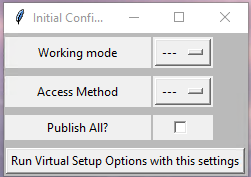
\includegraphics[width=0.6\linewidth]{Im/figures/proposed-work/bios-gui-initial-config}
        \caption{Menu to Select initial configuration for work}\label{fig:proposed-work-bios-gui-initial-config}
    \end{figure}
    
    \begin{figure}[htbp]
        \centering
        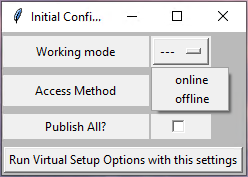
\includegraphics[width=0.6\linewidth]{Im/figures/proposed-work/bios-gui-initial-config-select-mode}
        \caption{Available work mode for the system: Online and Offline}\label{fig:proposed-work-bios-gui-initial-config-select-mode}
    \end{figure}

    \begin{figure}[htbp]
        \centering
        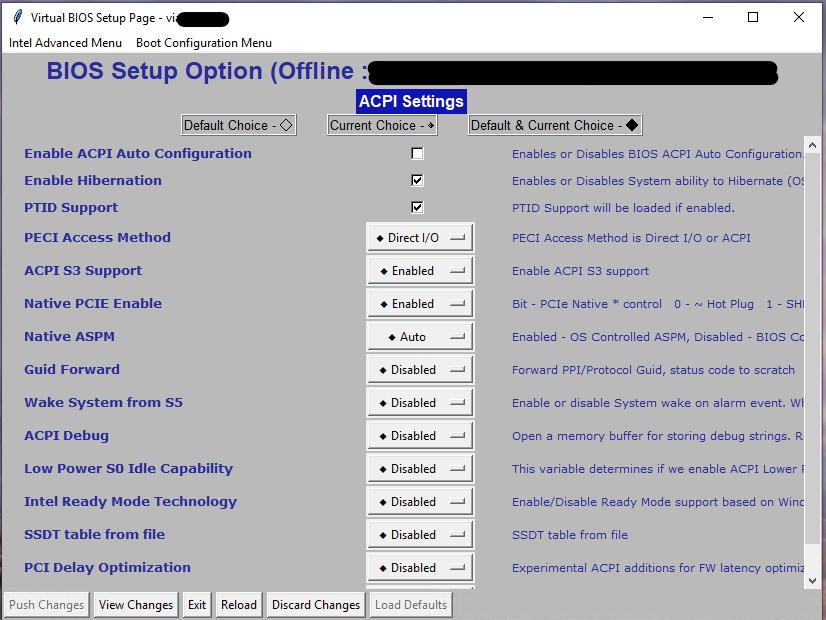
\includegraphics[width=0.6\linewidth]{Im/figures/proposed-work/bios-gui-acpi-knobs}
        \caption{Setup Options listed under ACPI Configurations}\label{fig:proposed-work-bios-gui-acpi-knobs}
    \end{figure}

    \begin{figure}[htbp]
        \centering
        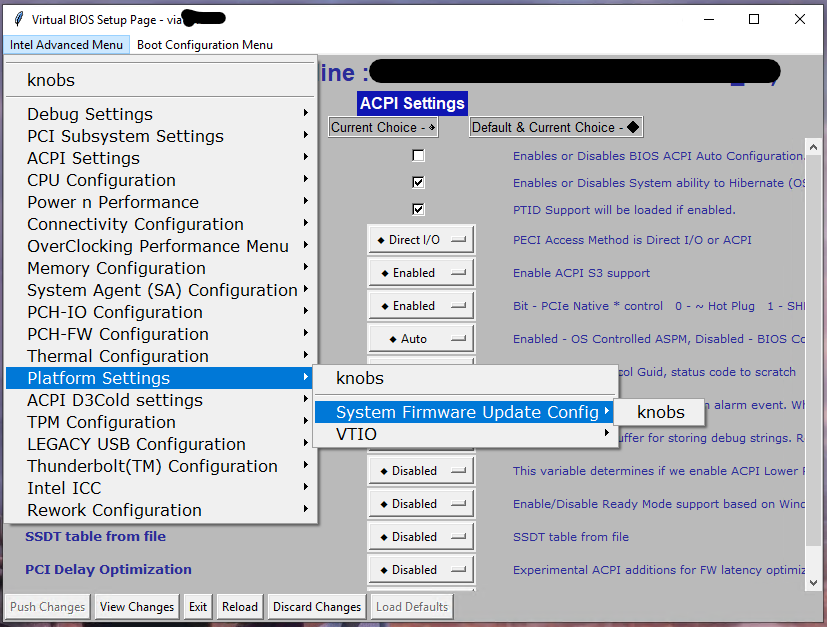
\includegraphics[width=0.6\linewidth]{Im/figures/proposed-work/bios-gui-accessing-menu}
        \caption{Navigating through BIOS setup page}\label{fig:proposed-work-bios-gui-accessing-menu}
    \end{figure}
\end{frame}

\subsubsection{Processing Firmware individually}
\begin{frame}{Primary Goals}
    \begin{itemize}
        \item Remove other Intellectual Property's dependency (\gls{ip} dependency) during firmware loading
        \item \gls{ip} Subsystem :
        \begin{itemize}
            \item Loader and Verifier
            \item \gls{ip} is always consumer
        \end{itemize}
        \item Signature verification using \gls{sha} hash algorithm and should be ease support for adding new algorithmic support as needed.
        \item Should support hardware based and software based verification support
        modifying memory requirements for given IP without impacting eco-system
        \item Prevent common security threats
        \item Allow easier OEM adoption and modification based on the respective design
        \item Reusability/Portability of design across many \gls{ip}s
        \item Generic design which supports any new IP integration
    \end{itemize}
\end{frame}

\begin{frame}{Structure of Module}
    \begin{figure}[htbp]
        \centering
        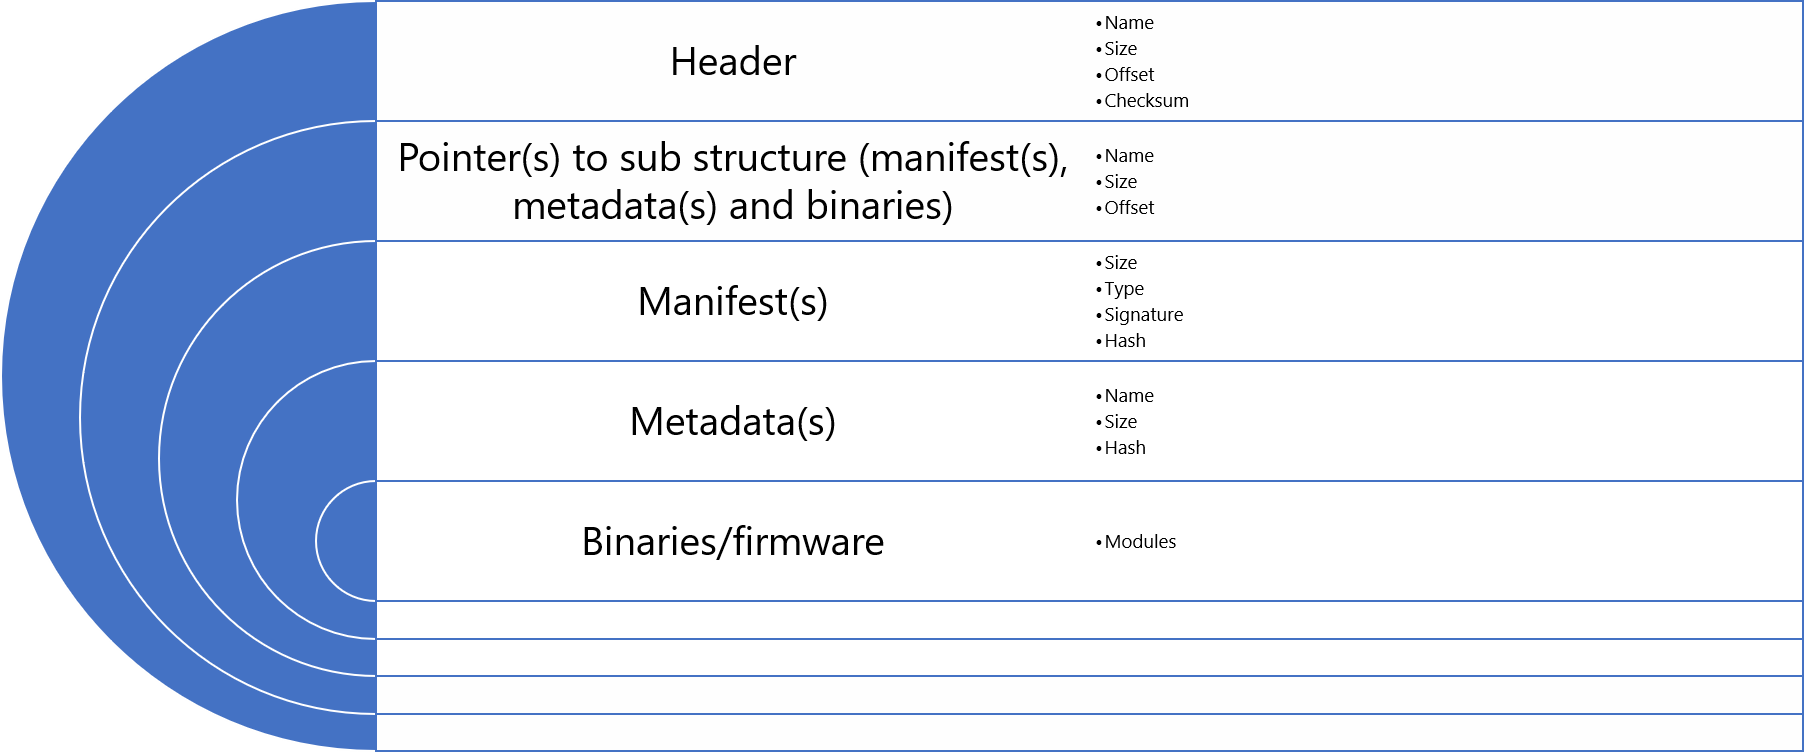
\includegraphics[width=\linewidth]{Im/figures/proposed-work/proposed-structure-firmware-signing}
        \caption{Proposed Structure for firmware signing}\label{fig:proposed-work-proposed-structure-firmware-signing}
    \end{figure}
\end{frame}

